\documentclass[oneside,14pt]{extarticle}
\usepackage[utf8]{inputenc}
\usepackage[english,ukrainian]{babel}
\usepackage{amssymb,amsfonts,amsmath,amsthm,mathtext,textcomp}
\usepackage{fontspec}
\setmainfont[Mapping=tex-text]{Times New Roman}
\usepackage[includehead, headsep=0pt, footskip=0pt, top=2cm, bottom=2cm, left=2cm, right=1cm]{geometry}
\usepackage{indentfirst}
\usepackage[onehalfspacing]{setspace}
\usepackage[headings]{fancyhdr}
\usepackage{etoolbox}
\usepackage{flafter}
\usepackage{listings}
\usepackage{graphicx}
\usepackage{float}
\usepackage[labelsep=period]{caption}
\lstset{
	breaklines=false
}
\usepackage{array}
\fancyhf{}
\renewcommand{\headrulewidth}{0pt}
\pagestyle{fancy}
\fancyfoot[R]{\thepage}
\lstset{breaklines=true,}
\graphicspath{ {./pictures} }

\lstset{
	language=c,
	tabsize=4,
	keepspaces,
	showstringspaces=false,
}
\graphicspath{ {./pictures} }
\setlength{\parindent}{4em}
\setlength\tabcolsep{5px}

\newcommand\subject{Моделювання та аналіз програмного забезпечення}
\newcommand\lecturer{доцент кафедри ПЗ \\ Сердюк П.В.}
\newcommand\teacher{викладач кафедри ПЗ \\ Микуляк А.В.}
\newcommand\mygroup{ПЗ-22}
\newcommand\lab{6}
\newcommand\theme{Дослідження предметної області та
	проектування системи за допомогою UML діаграм}
\newcommand\purpose{Дослідити предметну область та
	проектування системи за допомогою UML діаграм}

\begin{document}
\begin{normalsize}
	\begin{titlepage}
		\thispagestyle{empty}
		\begin{center}
			\textbf{МІНІСТЕРСТВО ОСВІТИ І НАУКИ УКРАЇНИ\\
				НАЦІОНАЛЬНИЙ УНІВЕРСИТЕТ "ЛЬВІВСЬКА ПОЛІТЕХНІКА"}
		\end{center}
		\begin{flushright}
			\textbf{ІКНІ}\\
			Кафедра \textbf{ПЗ}
		\end{flushright}
		\vspace{70pt}
		\begin{center}
			\textbf{ЗВІТ}\\
			до лабораторної роботи № \lab\\
			\textbf{на тему}: “\textit{\theme}”\\
			\textbf{з дисципліни}: “\subject”
		\end{center}
		\vspace{50pt}
		\begin{flushright}
			
			\textbf{Лектор}:\\
			\lecturer\\
			\vspace{10pt}
			\textbf{Виконав}:\\
			
			студент групи \mygroup\\
			Коваленко Д.М.\\
			\vspace{10pt}
			\textbf{Прийняв}:\\
			
			\teacher\\
			
			\vspace{28pt}
			«\rule{1cm}{0.15mm}» \rule{1.5cm}{0.15mm} 2023 р.\\
			$\sum$ = \rule{1cm}{0.15mm}……………\\
			
		\end{flushright}
		\vspace{\fill}
		\begin{center}
			\textbf{Львів — 2023}
		\end{center}
	\end{titlepage}
		
	\begin{description}
		\item[Тема.] \theme.
		\item[Мета.] \purpose.
	\end{description}

	\section*{Завдання}
Відповідно до завдання, яке ви виконуєте у рамках команди (3-4 студенти в команді)
розробити:
\begin{itemize}
	\item діаграму діяльності;
	\item діаграму класів (+- 10 класів для кожного студента).
\end{itemize}

Врахувати у проектах інтерактивну взаємодію користувачів. Всі діаграми повинні бути
складними, оскільки кінцевої реалізації проекту не потрібно, як і всіх задекларованих
можливостей у діаграмах.

Побудувати діаграму класів із використанням основних парадигм ООП. Для інкапсуляції
логіки, створити щонайменше 2 модулі: модуль з класами, що відповідальні за внутрішню
логіку програми (бізнес-логіку) та модуль інтерфейсу користувача. Модифікатори доступу
класів і полів повинні надавати доступ лише до необхідних елементів, усі решта повинні бути
невидимі розробнику інтерфейсу користувача.

Ролі у команді - TL:
\begin{itemize}
	\item Розробити діаграми компонент і розгортання. Спроектувати збірки: моделі,
	Unit тести, клієнта з графічним інтерфейсом (web, mobile, desktop). Якщо є
	необхідність то реалізувати інші збірки: сервера, іншого клієнт (наприклад
	може бути 2 клієнта – під веб та під мобільний пристрій).
\end{itemize}
	\section*{Хід виконання}
	\begin{figure}[H]
		\centering
		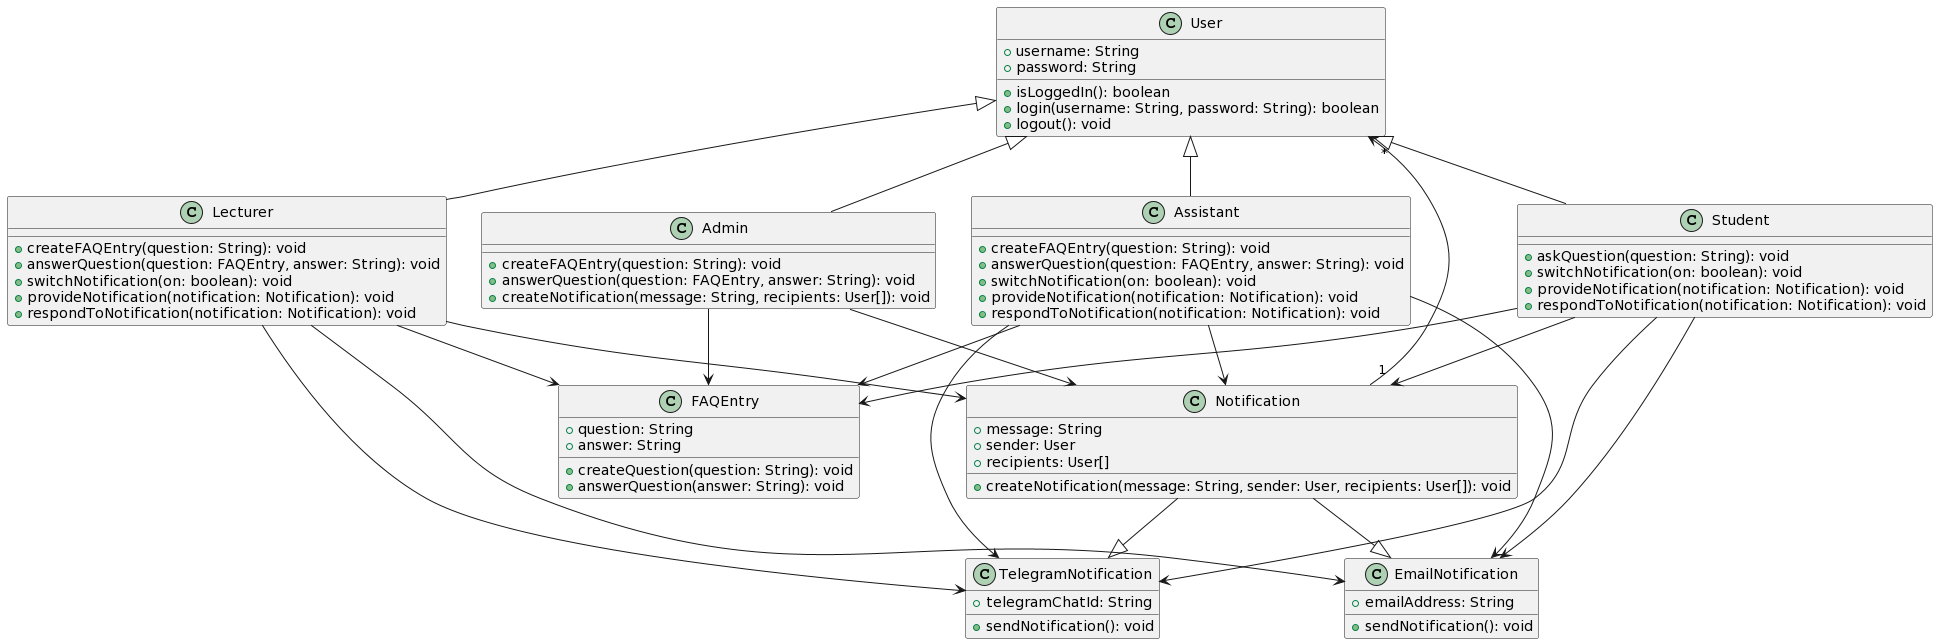
\includegraphics[width=\textwidth]{class}
		\caption{Діаграма класів виконанана відповідно до індивідуального варіанту}
	\end{figure}
	
	\begin{figure}[H]
		\centering
		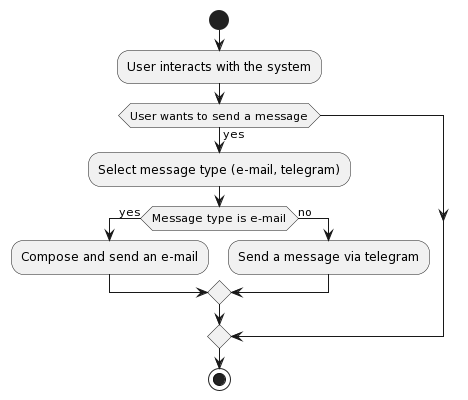
\includegraphics[width=0.55\textwidth]{activity1}\hfill
		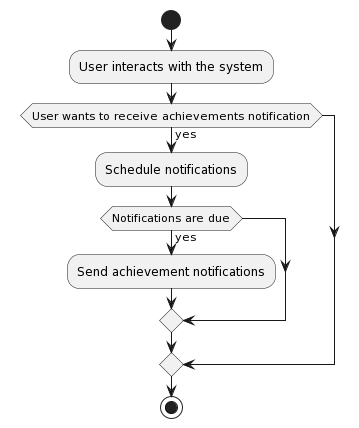
\includegraphics[width=0.4\textwidth]{activity2}\par
		\vspace{0.5cm}
		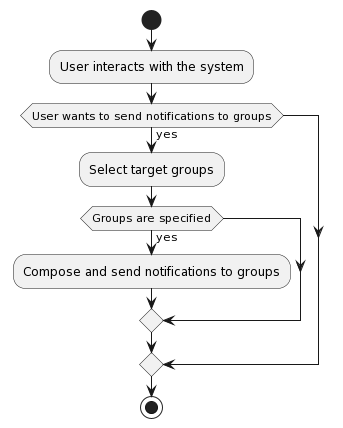
\includegraphics[width=0.4\textwidth]{activity3}\hfill
		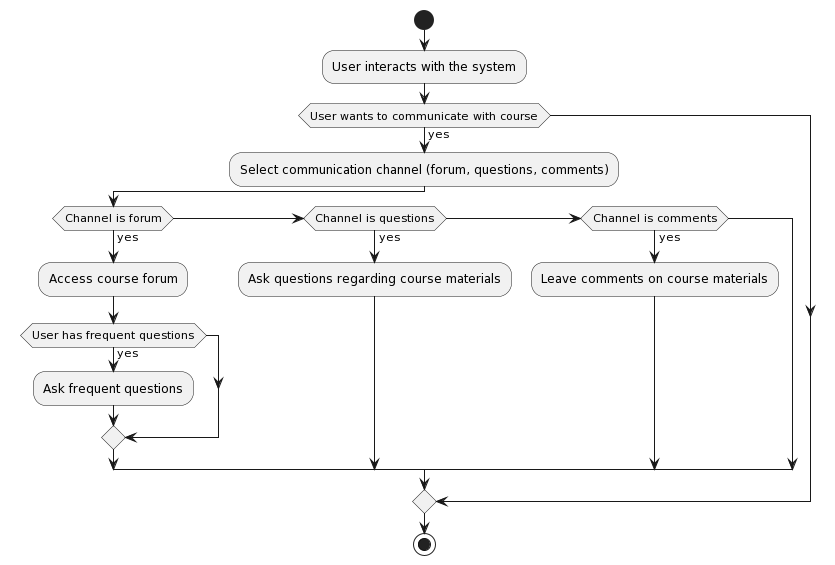
\includegraphics[width=0.6\textwidth]{activity4}\par
		\caption{Діаграми активності виконані відповідно до індивідуального варіанту}
	\end{figure}
	
	\begin{figure}[H]
		\centering
		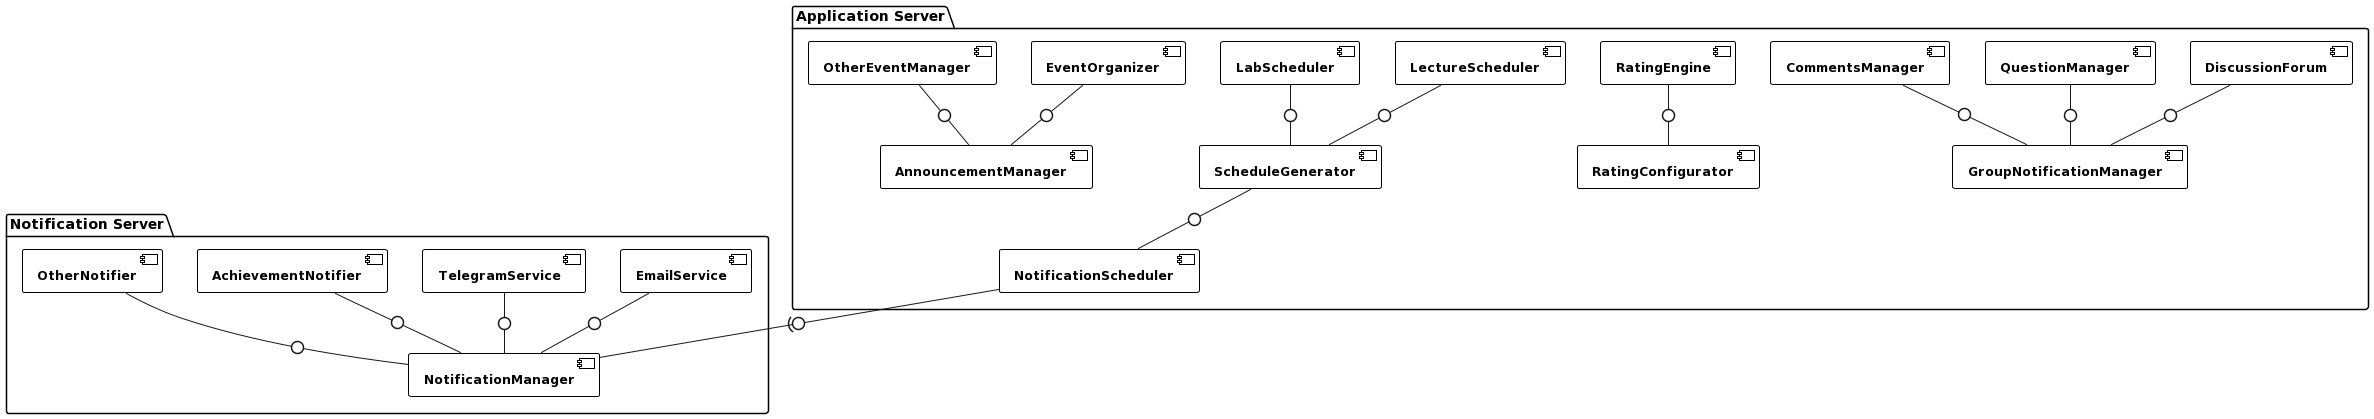
\includegraphics[width=\textwidth]{component}
		\caption{Діаграма компонентів виконана відповідно до ролі у команді}
	\end{figure}
	
	\begin{figure}[H]
		\centering
		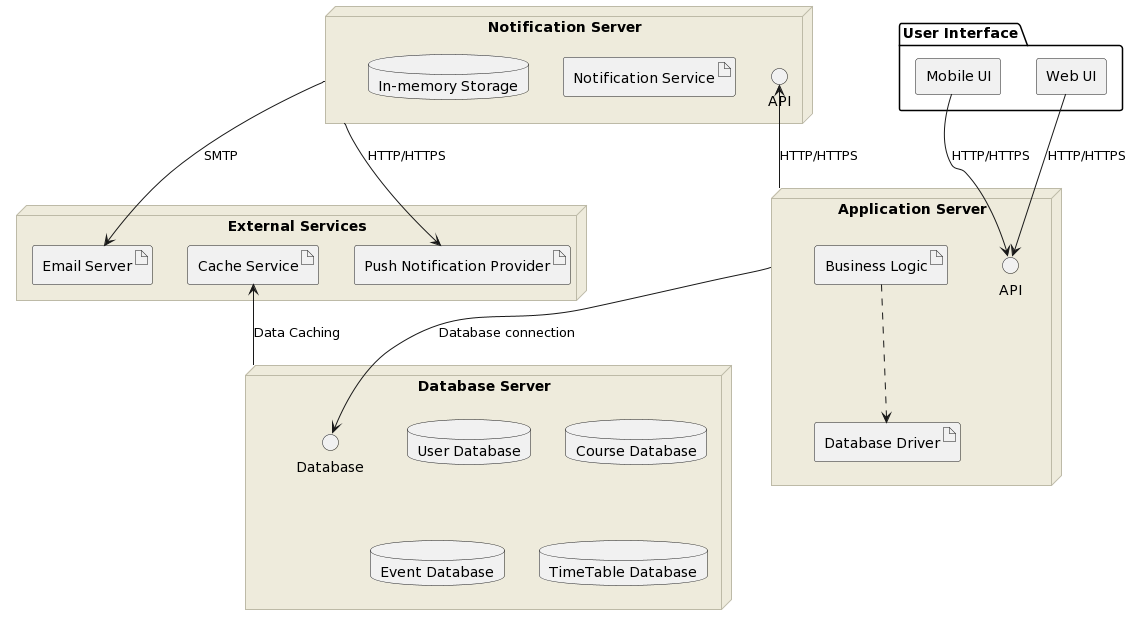
\includegraphics[width=\textwidth]{deployment}
		\caption{Діаграма розгортання виконана відповідно до ролі у команді}
	\end{figure}
	
	\begin{figure}[H]
		\centering
		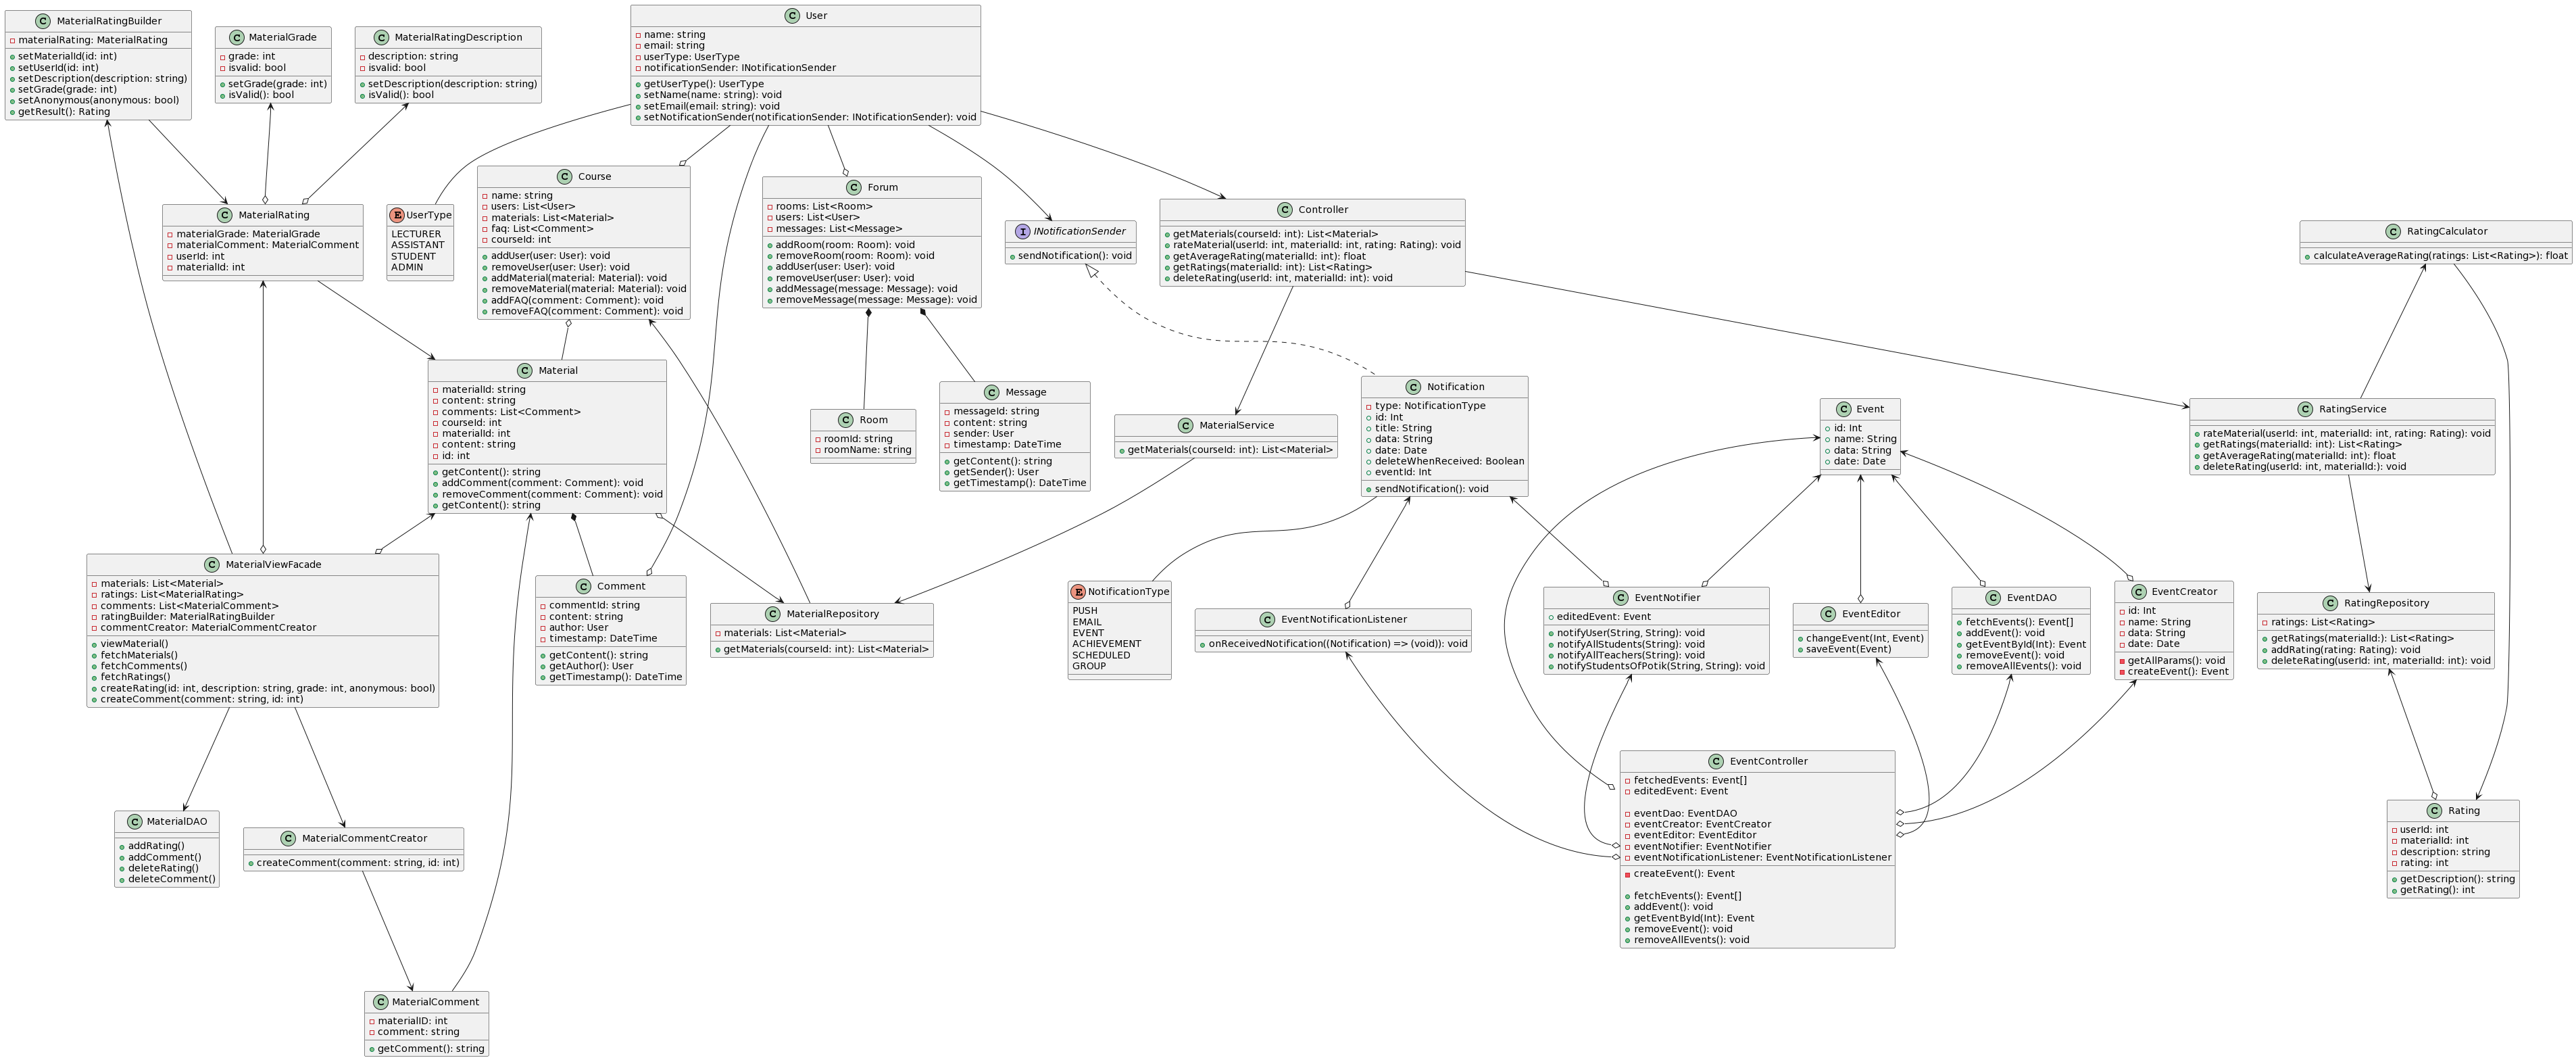
\includegraphics[width=\textwidth]{classes}
		\caption{Діаграма класів виконана відповідно до ролі у команді}
	\end{figure}
		
	\section*{Проектування збірок системи}
	\begin{itemize}
		\item Front-end: React.js.
		\item Mobile: React Native.
		\item Back-end: Node.js, Express.js, MongoDB.
		\item Розгортання: Docker, Kubernetes, AWS.
		\item Тестування: Jest.
	\end{itemize}
	
	Процес розгортання: Збірка фронтенду, бекенду та мобільного додатку, контейнеризація за допомогою Docker, розгортання кластеру Kubernetes на AWS, перед розгортанням виконання тестів з використанням Jest. Завантаження мобільного додатку у магазини мобільних додатків Google Play Store та Apple App Store.

	\section*{Висновки}
	   Під час виконання лабораторної роботи мною був проведений детальний аналіз предметної області та розроблена система за допомогою UML діаграм. Цей процес дозволив мені навчитись визначати вимоги до системи, її функціональність та структуру. Я зробив діаграми, що демонструють структуру та логіку проекту, зокрема взаємодію з користувачами. Це допомогло команді розуміти вимоги та функціональні можливості системи, а також сприяло подальшій розробці та розгортанню проекту.
\end{normalsize}
\end{document}
